\textcolor{blue}{Problem 2}
\begin{enumerate}
    \item From Figure 4.12, $\mathbb{E}[E_{out}(g^-_{m^*})]$ is initially decreasing. How can this be, if $\mathbb{E}[E_{out}(g^-_{m^*})]$ is increasing in $K$ for each $m$? (10pt)
    \item From Figure 4.12 we see that $\mathbb{E}[E_{out}(g^-_{m^*})]$ is initially decreasing, and then it starts to increase. What are the possible reasons for this? (10pt)
    \item When $K=1$, $\mathbb{E}[E_{out}(g^-_{m^*})]<\mathbb{E}[E_{out}(g_{m^*})]$. How can this be, if the learning curves for both models are decreasing? (10pt)
\end{enumerate}
\begin{figure}[htbp]
    \centering
    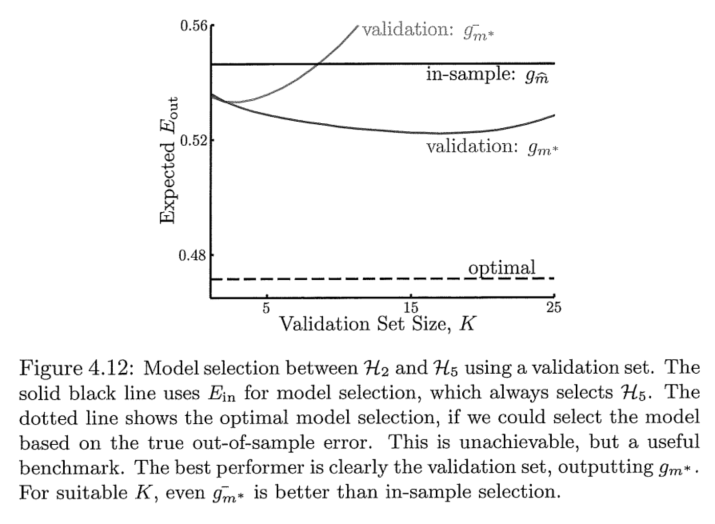
\includegraphics[width=0.8\textwidth]{../fig/figure412.png}
\end{figure} 
\par     
\textcolor{blue}{Solution}
















\newpage